\subsection{Analysis of \lemref{lem:analyticalSolutionK=2} for K=2}\label{sec:detectionBounds}
%Since the solution \eqref{eq:lambdaStarWeighted} for $K=2$ is an important building block in the
%approximate optimization of the outlier-robust objective \eqref{eq:outlierRobustObjective},
We now bound the probability that the solution as given by \lemref{lem:analyticalSolutionK=2} fails to detect the correct boundary. We use the derived bound to show that the weights given in \lemref{lem:weighted_solution_l0_l1} are optimal in a sense explained below.
For simplicity we analyze the one dimensional case $\vxii\in\mathbb{R}$, and we show later how the results generalize to multidimensional data.

We assume now that the data sequence is composed of two subsequences
of lengths $n_1$ and $n_2$, each composed of samples taken iid
from some probability distributions with means $\mu_1$
and $\mu_2$ respectively, and define $\Delta\mu\triangleq\mu_2-\mu_1$. We further
assume that the samples are bounded, i.e. $\abs{\vxii}\leq M/2,\;i=1\comdots n$,
for some positive constant $M$.
We set $w_i=1$ for all $i=1\comdots n-1$, and quote results for the weighted case where relevant. We note that $n_1$ and $n_2$ represent the
ground-truth, and not a variable we have to optimize.
We parameterize the sample-index argument of $g\paren{\cdot}$ in \eqref{eq:lambdaStarWeighted} as $i=n_1+m$ (and similarly $i^*=n_1+m^*$), that is we measure it
%We denote by $m$ the splitting point detected by the solution to \eqref{eq:lambdaStarWeighted}, measured
relatively to the true
splitting point $n_1$. For ease of notation, in what follows we substitute $g\paren{m}$ for $g\paren{n_1+m}$.
%Define the random variable
%$Y_m$ which is the difference between the empirical means of two
%subsequences created by splitting after $n_1+m$ samples:
%\begin{align}
%%    X_{k_1:k_2} &\triangleq \frac{1}{k_2-k_1+1}\sum_{i=k_1}^{k_2}\vxii\\ %\quad,\quad
%    Y_m &\triangleq\frac{1}{n_2-m}\negspaces\sum_{i=n_1+m+1}^{n}\negspace\vxii-\frac{1}{n_1+m}\sum_{i=1}^{n_1+m}\vxii.
%\end{align}
%This allows us to rewrite
%\eqref{eq:lambdaStarWeighted} as an optimization over $m$:
%\begin{align}\label{eq:optimal_m_star}
%    %\!\!\!\!g\paren{m} &\!\triangleq\! \frac{(n_1\!+\!m)(n_2\!-\!m)}{n}\abs{Y_m},\\ %\quad,\quad
%%    m^* \!=\!\argmax{m}{g\paren{m}},% \!\!\!%,%\nonumber
%    g\paren{m} &\triangleq \frac{(n_1+m)(n_2-m)}{n}\abs{Y_m},\\
%    m^* &=\argmax{m}\braces{g\paren{m}},\nonumber
%\end{align}
%where $m\in\brackets{-n_1+1,n_2-1}$.
Without loss of generality, we treat the case where
$m\geq0$. Note that $m^*\neq0$ if $g(0)<g(m)$ for some $m>0$.
%(it is not necessarily the optimal value $m^*$).
The probability of this event is bounded:
%\begin{align}\label{eq:correctBoundaryErrProb}
%    %\prob{g(0)<g(m)}=
%    \prob{\frac{n_1n_2}{n}\abs{Y_0}<\frac{(n_1+m)(n_2-m)}{n}\abs{Y_m}}.
%\end{align}
%Defining the following random variables:
%\begin{equation}\label{eq:Wdef}
%    W_m^{\pm}\triangleq\frac{n_1n_2}{n}Y_0\pm\frac{(n_1+m)(n_2-m)}{n}Y_m,
%\end{equation}
%it holds that
\begin{align}\label{eq:1D_errBound_m}
    \prob{g(0)<g(m)} %& \leq\prob{W_m^{+}<0}+\prob{W_m^{-}<0}\\
    %& \leq 2\prob{W_m^{-}<0}
    \leq 2\exp\paren{-Cm},%\nonumber
\end{align}
for $C=\paren{2\Delta\mu^2n_1^2}/\paren{M^2n^2}$.
The proof is given in %\secref{sec:proof:1D_errBound_m} of
the supplementary material.
% of \cite{DBLP:journals/corr/LattimoreCS14}.

Note that in order for the bound to be useful, the true segments should not be
too long or too short, in agreement with the motivation for using weights given
before \lemref{lem:weighted_solution_l0_l1}.
We now use \eqref{eq:1D_errBound_m} to prove the following theorem:
\begin{theorem}\label{thm:1D_errBound}
    Consider a sequence of $n$ variables as described
    above. Given $\delta\in(0,1)$ set
    $m_0=\frac{\log\paren{2n_2/\delta}}{C}$. Then, the probability that
    the solution %$m^*$ to \eqref{eq:optimal_m_star}
    $i^*=n_1+m^*$ as given in \lemref{lem:analyticalSolutionK=2} %to \eqref{eq:lambdaStarWeighted}
    is no less than
    $m_0$ samples away from the true boundary is bounded,
    $\mathbb{P}\paren{m^*\geq m_0}\leq\delta$~.
\end{theorem}
The proof appears in %\secref{sec:proof:1D_errBound} of
the supplementary material.
% of \cite{DBLP:journals/corr/LattimoreCS14}.

Considering the weighted case with arbitrary $w_i$, we repeated the calculation for the bound on
%$\prob{W_m^{-}<0}$ which is the quantity of interest.
$\prob{g(0)<g(m)}$.
To illustrate the influence of the weights on the bound, we heuristically parameterize $w_j=\paren{j\paren{n-j}}^\alpha$ for some $\alpha\in\brackets{0,1}$\footnote{This parametrization is motivated by \eqref{eq:lambdaStarWeighted}}.
%Repeating the calculation for arbitrary weights $w_i$, we derive the following bound on $\prob{W_m^{-}<0}$ which is the quantity
%of interest:
%\begin{align}\label{eq:weighted_bound}
%    \prob{W_m^{\pm}<0}= \exp(-\nu/\delta)
%\end{align}
%where
%\begin{align*}
%\nu &= 2n_1^2\Delta\mu^2\paren{c_{n_1}n_2\pm
%  c_{n_1+m}\paren{n_2-m}}^2\\
%\delta &= M^2n\Bigg(\pm2c_{n_1}c_{n_1+m}n_1\paren{n_2-m}\\&+c_{n_1}^2n_1n_2+c_{n_1+m}^2\paren{n_1+m}\paren{n_2-m}\Bigg)~,
%\end{align*}
%and $c_j\triangleq\frac{1}{w_j}$.
%Based on \eqref{eq:lambdaStarWeighted}, we heuristically set $w_j=\paren{j\paren{n-j}}^\alpha$ for some $\alpha\in\brackets{0,1}$.
%As for the unweighted case, it is enough to bound $\prob{W_m^-<0}$, as it is an upper bound of the bound for $\prob{W_m^+<0}$. As mentioned above, for the unweighted case, $c_j=1$, $j=1,\ldots,n-1$, the bound \eqref{eq:weighted_bound} decays faster as a function of $m$ if $n_1\approx n_2$, when compared to $n_1\ll n_2$.
%In order to achieve a better decay rate even for $n_1\ll n_2$, we set $w_j=\paren{j\paren{n-j}}^\alpha$.
The bound as a function of $m$ is illustrated in \figref{fig:weighted_bounds} for several values of $\alpha$.
It is evident that indeed $\alpha>0$ achieves a faster decaying bound for small $n_1$, and that $\alpha=0.5$ is optimal in the sense that for $\alpha>0.5$ the bound is no longer a monotonous function of $m$. This agrees with the weights given by \lemref{lem:weighted_solution_l0_l1}. We note that this specific choice of the weights was derived as well by \cite{bleakley2011group} by assuming a Gaussian noise model, while our derivation is more general.
%While it is evident that for
%$n_1\approx n_2$ (\figref{fig:weighted_bounds4}) and $m>20$ the bound
%for $\alpha=0.5$ is less tight than the bound for $\alpha=0$, we note
%that the bound is already quite small for these values of $m$,
%typically less than $10^{-2}$, such that the overall advantage of setting
%$\alpha\neq0$ is significant.
%-----------------------------------------
\begin{figure}[!t]
        \begin{minipage}{.47\textwidth}
            \newcommand{\factor}{.49} %\newcommand{\factor}{.49}
            \centering
            %\subfigure[$n_1=10$\label{fig:weighted_bounds1}]{\includegraphics[width=\factor\linewidth]{figures/bounds_weights1}}
            \subfigure[$n_1=20$\label{fig:weighted_bounds2}]{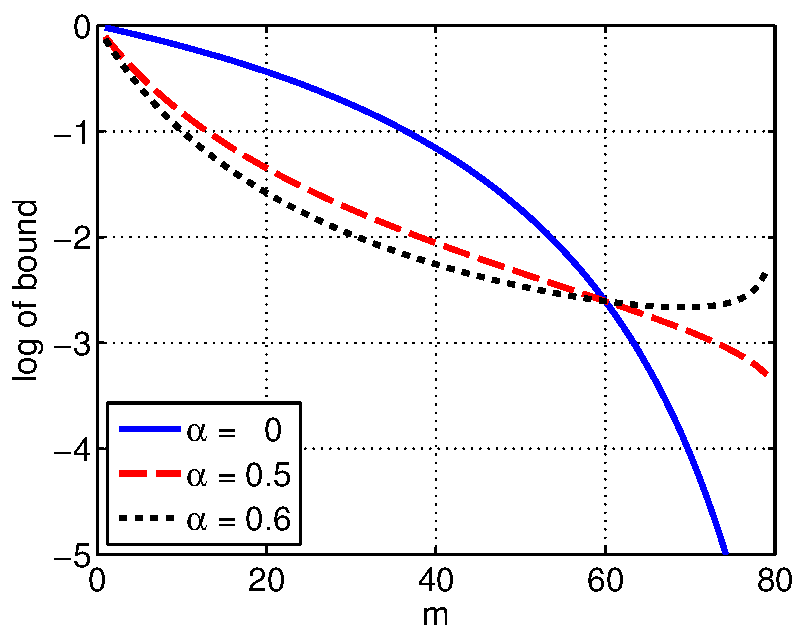
\includegraphics[width=\factor\linewidth]{figures/orig_in_color/bounds_weights_n20}}
            %\subfigure[$n_1=30$\label{fig:weighted_bounds3}]{\includegraphics[width=\factor\linewidth]{figures/bounds_weights3}}
            \subfigure[$n_1=40$\label{fig:weighted_bounds4}]{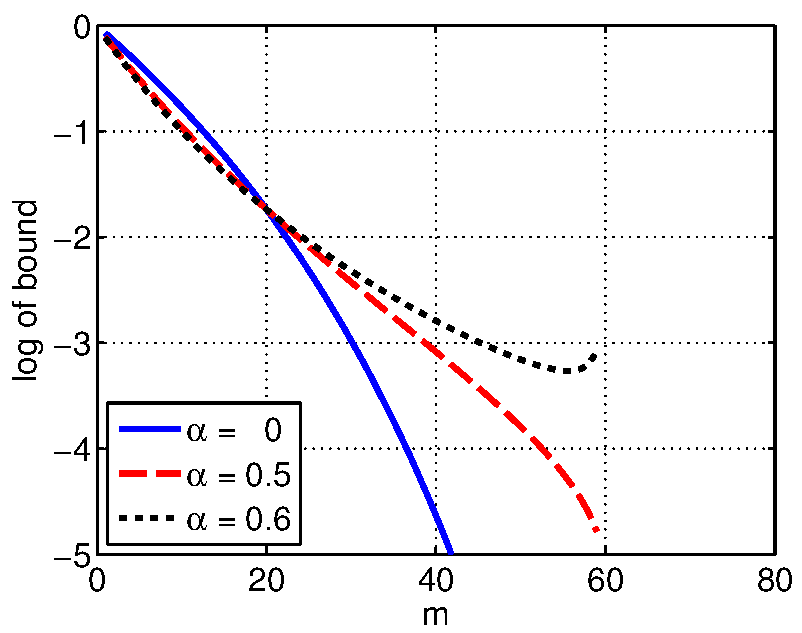
\includegraphics[width=\factor\linewidth]{figures/orig_in_color/bounds_weights_n40}}
            \caption{Bounds on %the probability
            %$\prob{W_m^-<0}$
            $\prob{g(0)<g(m)}$
            as a function of the distance $m$ from the true boundary $n_1$, for $n=100$, two values of $n_1$, and various values of the weighting parameter $\alpha$. The case of $\alpha=0$ amounts to uniform weights.}\label{fig:weighted_bounds}
            \quad
            \renewcommand{\factor}{.6}
            \centering
            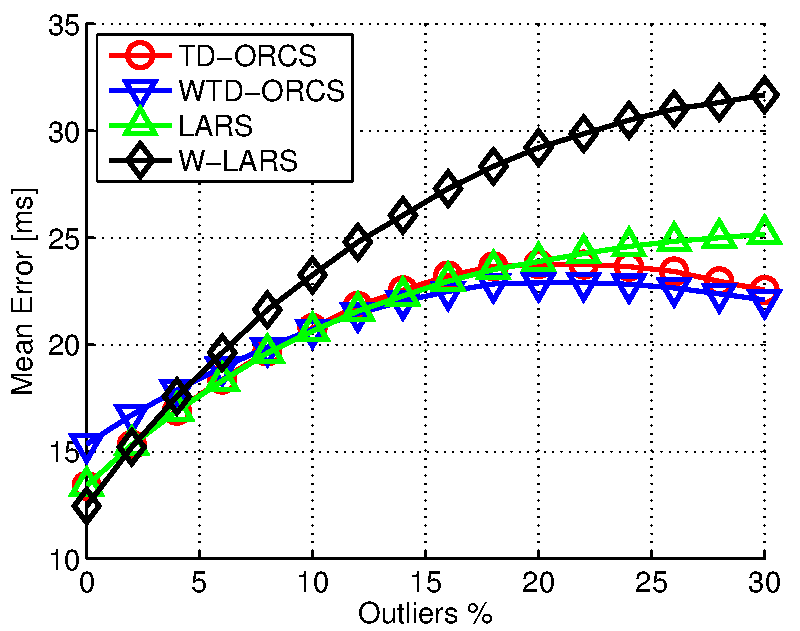
\includegraphics[width=\factor\linewidth]{figures/orig_in_color/biphonesSeg_robust}
            \caption{Mean error (absolute time difference to ground-truth boundary)
            of four algorithms on TIMIT phonetic data contaminated with outliers. See text for a list of algorithms compared.}\label{fig:biphonesSeg_robust}
        \end{minipage}
\end{figure}
%\end{wrapfigure}
%-----------------------------------------
% \begin{figure*}[!t]
%         \newcommand{\factor}{.24}
%         \centering
%         \begin{subfigure}{\factor\linewidth}
%                 \includegraphics[width=\linewidth]{figures/bounds_weights1}
%                 \caption{$n_1=10$}\label{fig:weighted_bounds1}
%         \end{subfigure}
%         \begin{subfigure}{\factor\linewidth}
%                 \includegraphics[width=\linewidth]{figures/bounds_weights2}
%                 \caption{$n_1=20$}\label{fig:weighted_bounds2}
%         \end{subfigure}
%         \begin{subfigure}{\factor\linewidth}
%                 \includegraphics[width=\linewidth]{figures/bounds_weights3}
%                 \caption{$n_1=30$}\label{fig:weighted_bounds3}
%         \end{subfigure}
%         \begin{subfigure}{\factor\linewidth}
%                 \includegraphics[width=\linewidth]{figures/bounds_weights4}
%                 \caption{$n_1=40$}\label{fig:weighted_bounds4}
%         \end{subfigure}
%        \caption{Bounds on the probability $\prob{W_m^-\leq0}$ as a function of distance $m$ from the true boundary $n_1$, for various values of $n_1$ and
%        various values of the weighting parameter $\alpha$. The case of $\alpha=0$ amounts to uniform weights (i.e., no weighting).}
%        \label{fig:weighted_bounds}
% \end{figure*}
%
Finally, we note that generalizing the results for multidimensional
data is done by using the fact that for any two vectors
$a,b\in\mathbb{R}^d$, it holds true that
$\prob{\vnorm{a}_2\leq\vnorm{b}_2}\leq\sum_i\prob{\abs{a_i}\leq\abs{b_i}}$. Thus
generalizing
%\eqref{eq:correctBoundaryErrProb}
\eqref{eq:1D_errBound_m}
for $d>1$ is
straightforward. While the bound derived in this way will have a
multiplicative factor of the dimension of the data $d$, it is still
exponential in the number of samples $n$.
%Deriving a bound which is independent of $d$ is left to future work.
